% Preámbulo
\documentclass[stu, 12pt, letterpaper, donotrepeattitle, floatsintext]{apa7}
\usepackage[utf8]{inputenc}
\usepackage{comment}
\usepackage{marvosym}
\usepackage{graphicx}
\usepackage{float}
\usepackage{listings}
\usepackage{color}
\usepackage{fancyvrb} % for "\Verb" macro
\usepackage{amsmath}
%Includes "References" in the table of contents
\usepackage[nottoc]{tocbibind}
\usepackage[normalem]{ulem}
\usepackage[spanish]{babel} 
\usepackage{indentfirst} %para le formato que quiere la profe QUITAR SI QUIERES OG APA7
\usepackage{ragged2e} %para le formato que quiere la profe QUITAR SI QUIERES OG APA7
\usepackage{indentfirst} %para le formato que quiere la profe QUITAR SI QUIERES OG APA7

\renewcommand\labelitemi{$\bullet$}

\definecolor{mygreen}{rgb}{0,0.6,0}
\definecolor{mygray}{rgb}{0.5,0.5,0.5}
\definecolor{mymauve}{rgb}{0.58,0,0.82}
 
%Customize a bit the look
\lstset{ %
backgroundcolor=\color{white}, % choose the background color; you must add \usepackage{color} or \usepackage{xcolor}
basicstyle=\footnotesize, % the size of the fonts that are used for the code
breakatwhitespace=false, % sets if automatic breaks should only happen at whitespace
breaklines=true, % sets automatic line breaking
captionpos=b, % sets the caption-position to bottom
commentstyle=\color{mygreen}, % comment style
deletekeywords={...}, % if you want to delete keywords from the given language
escapeinside={\%*}{*)}, % if you want to add LaTeX within your code
extendedchars=true, % lets you use non-ASCII characters; for 8-bits encodings only, does not work with UTF-8
frame=single, % adds a frame around the code
keepspaces=true, % keeps spaces in text, useful for keeping indentation of code (possibly needs columns=flexible)
keywordstyle=\color{blue}, % keyword style
% language=Octave, % the language of the code
morekeywords={*,...}, % if you want to add more keywords to the set
numbers=left, % where to put the line-numbers; possible values are (none, left, right)
numbersep=5pt, % how far the line-numbers are from the code
numberstyle=\tiny\color{mygray}, % the style that is used for the line-numbers
rulecolor=\color{black}, % if not set, the frame-color may be changed on line-breaks within not-black text (e.g. comments (green here))
showspaces=false, % show spaces everywhere adding particular underscores; it overrides 'showstringspaces'
showstringspaces=false, % underline spaces within strings only
showtabs=false, % show tabs within strings adding particular underscores
stepnumber=1, % the step between two line-numbers. If it's 1, each line will be numbered
stringstyle=\color{mymauve}, % string literal style
tabsize=2, % sets default tabsize to 2 spaces
title=\lstname % show the filename of files included with \lstinputlisting; also try caption instead of title
}
%END of listing package%
 
\definecolor{darkgray}{rgb}{.4,.4,.4}
\definecolor{purple}{rgb}{0.65, 0.12, 0.82}
 
%define Javascript language
\lstdefinelanguage{JavaScript}{
keywords={typeof, new, true, const, let,false, catch, function, return, null, catch, switch, var, if, in, while, ,for, do, else, case, break},
keywordstyle=\color{blue}\bfseries,
ndkeywords={class, export, boolean, throw, implements, import, this},
ndkeywordstyle=\color{darkgray}\bfseries,
numberstyle=\footnotesize,
identifierstyle=\color{black},
sensitive=false,
comment=[l]{//},
morecomment=[s]{/*}{*/},
commentstyle=\color{purple}\ttfamily,
stringstyle=\color{red}\ttfamily,
morestring=[b]',
morestring=[b]"
}
 
\lstset{
language=JavaScript,
extendedchars=true,
basicstyle=\footnotesize\ttfamily,
showstringspaces=false,
showspaces=false,
numbers=left,
numberstyle=\footnotesize,
numbersep=9pt,
tabsize=2,
breaklines=true,
showtabs=false,
captionpos=b
}

% Portada
%\thispagestyle{empty}
\title{\Large Atractores Caóticos para Producir Arte Generativo}
\author{María G. Bañuelos H.\: 19211640 \\
  Abraham J. Flores A.\: 19211640 \\
  Víctor M. Sánchez D.\: 19211732} % (autores separados, consultar al docente)
% Manera oficial de colocar los autores:
%\author{Autor(a) I, Autor(a) II, Autor(a) III, Autor(a) X}
\affiliation{Tecnológico Nacional de México | Instituto Tecnológico de Tijuana}
\course{SCC-1010SC5C Graficación}
\professor{Dra. Martha Elena Pulido}
\duedate{1 de diciembre de 2021}

\begin{document}
    % Índices
    \pagenumbering{arabic}
    \begin{figure}[ht]
      \centering
      
\includegraphics[width=16cm]{logosITT.png}
    \end{figure}
    \maketitle

    %indice
    \tableofcontents 
    \listoffigures

    % Cuerpo 
    %NOTA: PARA CITAR ESTILO "Merts (2003)" usar \cite{<nombre_cita_bib>}
    %    
    \newpage
    \section*{Introducción}
    \addcontentsline{toc}{section}{Introducción}
    En \begin{justifying}
      el estudio de sistemas como aquellos de la Ingeniería en Sistemas Computacionales, nos encontramos con el tema
    de los Sistemas Dinámicos que son sistemas que cambian a través del tiempo \cite{Meiss:2007} y buscan un punto de equilibrio \cite{unknown-author-2020}. Si se agregan
    más variables a estos sistemas de interés, tienden a acomplejarse resultando en Sistemas Dinámicos Complejos donde encontramos
    a un conjunto de sistemas que resultan en trayectorias cautivadoras aparentemente impredecibles dependiendo de las condiciones iniciales del sistema.
    Estos se llaman Atractores Caóticos \cite{bradley-2010}.\par
    \end{justifying}
    Con \begin{justifying}
      el avance exponencial de la tecnología y del Intenet, se han desarrollado y publicado temas variados \cite{kemp-2017}, tales como los Atractores Caóticos, así como
    el Arte Generativo, que ha ganado popularidad en los últimos años por ser un estilo de obras de arte generadas por procedimientos automatizados como los estudiados
    en las ingenierías y que se caracterízan por tener patrones geométricos \cite{unknown-author-no-date}\cite{lamine-2021}. Si se desarrolla una manera de utilizar lo cáotico de los sistemas dinámicos y 
    la visión artística para generar una obra única a partir de los atractores, nos permitiría estudiar ámbas disciplinas como solidos complementos de ámbos, reducír la barrera de entrada
    para las artes visuales, así como utilizar a estos sistemas para crear colecciones de NFT's que permiten la apertura del mercado artístico a los intereados en este estilo. En este proyecto, explicamos una
    manera de utilizar a los Atractores Caóticos para producir obras de Arte Generatívo y posibles rutas de monetización para las obras creadas.\par
    \end{justifying}
    \vspace{\baselineskip}
    \section*{Descripción del Proyecto}
    \addcontentsline{toc}{section}{Descripción del Proyecto}
    El \begin{justifying}
      nombre del proyecto es: \textbf{``Atractores Caóticos para Producir Arte Generativo''}. Consiste en utilizar
      uno de los atractores caóticos llamado \emph{Atractor De Lorenz}, graficar el movimiento de su trayectoria por medio del
      \emph{Método de Euler} junto con la librería del lenguaje JavaScript orientada a gráficos computarizados web \emph{Processing} y dentro del código desarrollado con esta librería, utilizar
      una función que genera un rectangulo como el adorno característico para la obra en cuestión, el cuál se ejecuta en los buscadores
      web que manejen lenguaje JavaScript. La idea está representada en la portada del video (Figura ~\ref{fig:video}). %citar a la figura 1
      \par
    \end{justifying}
    \begin{figure}[H]
      \centering
      \caption{Portada del video.}
      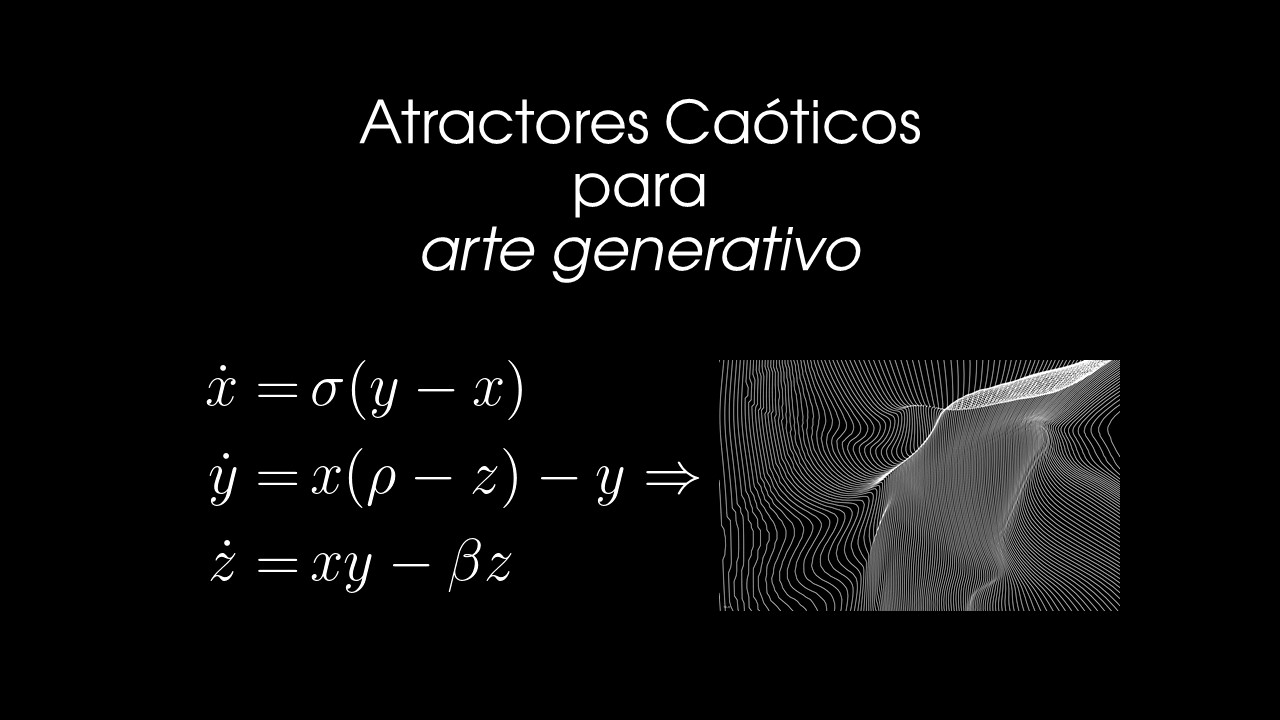
\includegraphics[width=10cm,height=6cm]{Thumbnail_Ecuaciones.jpg}
      \\\emph{Nota:} Autoría propia.\label{fig:video}
    \end{figure}
    \section*{Objetivos}
    \addcontentsline{toc}{section}{Objetivos}
    \begin{itemize}
      \item Utilizar el Atractor de Lorenz como generador de valores para producir obras de arte generativo.
      \item Explicar el concepto del Arte Generativo y las corrientes artísticas que lo influyen.
      \item Explicar el concepto de los Sistemas Dinámicos y las características del Atractór de Lorenz.
      \item Documentar las etapas del proceso de la obra resultante como precedente para futuros métodos de producción de arte generativo.
      \item Mostrar las capacidades de la librera \emph{Processing} como herramienta auxiliar para la graficación computarizada.
    \end{itemize}\par
    \vspace{\baselineskip}
    \section*{Planteamiento del Problema}
    \addcontentsline{toc}{section}{Planteamiento del Problema}
    Para \begin{justifying}
      las personas interesadas en la creación de arte digital que no disponen de habilidades de dibujo y de manejo de programas de edición digital por los costos
      de sus membresias de uso se enfrentan con una barrera de entrada muy grande a este rubro. Con los conocimientos básicos de \emph{Processing} y de la noción de Sistemas Dinámicos
      se les permite una opción relativamente sencilla para que incursionen en las artes visuales sin necesidad de ser buenos dibujantes.\par
    \end{justifying}
    Con \begin{justifying}
      este proyecto esperamos recabar la información necesaria para entender el método de producción expuesto y que lo puedan implemenar
      en sus estudios artístico-visuales.\par
    \end{justifying}
    \vspace{\baselineskip}
    \subsection*{Definición del Problema}
    \addcontentsline{toc}{subsection}{Definición del Problema}
    Teniendo el conocimiento de las trayectoras de los atractores caóticos, así como un conocimiento
    elemental de programación, el aplicar Atractores Caóticos en la creación del arte generativo ofusca el 
    desarrollo artístico de dichas herramientas.\par
    \vspace{\baselineskip}
    \section*{Justificación}
    \addcontentsline{toc}{section}{Justificación}
    A \begin{justifying}
      pesar de que se tiene una documentación extensa de los Sistemas Dinámicos tales como el Atractor de Lorenz, existe
      muy poca información especifica de las aplicaciones artísticas de dichos sistemas para producir obras de arte generativo, aparte de que 
      muchos artístas no deciden compartír los procedimientos de sus obras de mayor calídad por miedo a la plagiarización de sus trabajos. Esto
      ocasiona que los aspirantes a artísticas de arte generativo no tengan mucho material fuente con el cuál comenzar su camino, por lo que
      el documentar todo el proceso de este proyecto permite cerrar la brecha técnica como fuente de información y fuente de inspiración por
      las infinitas posibilidades que ofrecen los objetos de estudio en este mismo documento.\par
    \end{justifying}
    \vspace{\baselineskip}
    \section*{Diseño del Proyecto}
    \addcontentsline{toc}{section}{Diseño del Proyecto}
    La \begin{justifying}
      animación realizada es una animación 3D que contiene figuras geométricas 2D, que en conjunto se giran en dos ejes tridimensionales
    para hacer una ilusión de adimesionalidad geométrica. A continuación se explican las partes que lo conforman.\par
    \end{justifying}
    \vspace{\baselineskip}
    \subsection*{Atractor de Lorenz}
    \addcontentsline{toc}{subsection}{Atractor de Lorenz}
    Este \begin{justifying}
      es un modelo de las ecuaciones de Navier-Stokes que describen el movimiento de un fluido. Lorenz propuso un modelo para la predicción del clima
    a travéz del tiempo considerando las ecuaciones anteriores por lo que el sistema de Lorenz se describe de la siguiente manera:\par
    \end{justifying}
    \vspace*{-\abovedisplayskip}
    \begin{equation*}
      \begin{aligned}
        \frac{dx}{dt}&=\sigma (y-x)\\
        \frac{dy}{dt}&=(\rho-z)-y\\
        \frac{dz}{dt}&=xy-\beta z\\
      \end{aligned}
    \end{equation*}\par
    Para \begin{justifying}
      simplificar la escritura, se utiliza la notación punto de Newton que cambia los diferenciales por un punto escrito arriba de la función, que resulta en lo siguiente:\par
    \end{justifying}
    \vspace*{-\abovedisplayskip}
    \begin{equation*}
      \begin{aligned}
        \dot{x}&=\sigma (y-x)\\
        \dot{y}&=(\rho-z)-y\\
        \dot{z}&=xy-\beta z
      \end{aligned}
    \end{equation*}\par
    En \begin{justifying}
      este caso \(\sigma, \rho\) y \(\beta\) son constantes que se pueden elegir como se plazca. Para este proyecto se utilizaron los valores canónicos de Lorenz, los cuales
      son \(\sigma=28, \rho=10 \) y \(\beta=\frac{8}{3}\).\par
    \end{justifying}
    \vspace{\baselineskip}
    \subsection*{Método de Euler}
    \addcontentsline{toc}{subsection}{Método de Euler}
    Simplemente \begin{justifying}
      es un método numérico que permite calcular numéricamente los valores de una ecuación diferencial. Esto es de extrema utilidad ya que la conversión de las ecuaciones diferenciales
    analíticas a su equivalente numérico nos permite computarlo por medio de una computadora. Empezando por la notación analítica general de una ecuación diferencial, podemos llegar a su equivalente
    del Método de Euler, recordando que:\par
    \end{justifying}
    \vspace*{-\abovedisplayskip}
    \[\dot{y}=\lim_{h\rightarrow 0}{f(x+h)-f(x) \over h}\]\par
    Como \begin{justifying}
      queremos discretizar dicha ecuación, descartamos el límite.\par
    \end{justifying}
    \vspace*{-\abovedisplayskip}
    \[\dot{y}\approx{f(x+h)-f(x) \over h}\]\par
    Ahora \begin{justifying}
      resolvemos para \(f(x+h)\).\par
    \end{justifying}
    \vspace*{-\abovedisplayskip}
    \begin{equation*}
      \begin{aligned}
        \dot{y}&\approx{f(x+h)-f(x) \over h}\\
        h\cdot\dot{y}&\approx f(x+h)-f(x)\\
        h\cdot\dot{y}+f(x)&\approx f(x+h)\\
        f(x+h)&\approx f(x)+h\cdot\dot{y}
      \end{aligned}
    \end{equation*}\par
    Como \begin{justifying}
      estamos queriendo convertir una expresión analítica a su equivalente numerico, agregamos subíndices acorde a que: \par
    \end{justifying}
    \vspace*{-\abovedisplayskip}
    \begin{equation*}
      \begin{aligned}
        h&=x_{n+1}-x_n\\
        x_{n+1}&=x_n+h
      \end{aligned}
    \end{equation*}\par
    Y \begin{justifying}
      que:\par  
    \end{justifying}
    \vspace*{-\abovedisplayskip}  
    \[\dot{y}=\dot{y}(x)\]\par
    Entonces \begin{justifying}
      el Método Euler resulta en:\par
    \end{justifying}
    \vspace*{-\abovedisplayskip}
    \[f(x_{n+1})\approx f(x_n)+h\cdot\dot{y}(x_n)\]\par
    Donde \begin{justifying}
      \(h\) es un incremento generalmente diminuto.\par
    \end{justifying}
    \vspace{\baselineskip}
    \subsection*{Discretización del Atractor de Lorenz}
    \addcontentsline{toc}{subsection}{Discretización del Atractor de Lorenz}
    Con lo \begin{justifying}
      anterior, solo nos queda convertir al Atractor de Lorenz en su homólogo numérico.\par
    \end{justifying}
    \vspace*{-\abovedisplayskip}
    \begin{equation*}
      \begin{matrix}
        \dot{x}=\sigma (y-x)\\
        \dot{y}=(\rho-z)-y\\
        \dot{z}=xy-\beta z
      \end{matrix}\;\rightarrow\;
      \begin{matrix}
        x_{n+1}=x_n+h\cdot\sigma (y-x)\\
        y_{n+1}=y_n+h\cdot((\rho-z)-y)\\
        z_{n+1}=z_n+h\cdot(xy-\beta z)
      \end{matrix}
    \end{equation*}\par
    \subsection*{Código empleado}
    \addcontentsline{toc}{subsection}{Código empleado}
    El \begin{justifying}
      nombre del archivo es \verb|Origins_of_Symmetry.js|; la primer parte corresponde al título de la animación, que en parte
    está inspirada en la portada del 2do. disco de la banda Muse (Figura ~\ref{fig:muse}), %citar a la figura 2 
    que tiene el mismo nombre. La terminación \verb|.js| es para denotar que dicho archivo es del lenguaje JavaScript y que 
    la libreria de Processing pueda entender las sentencias dentro de éste.\par
    \end{justifying}
    \begin{figure}[H]
      \centering
      \caption{Portada del album Origins of Symmetry de Muse.}
      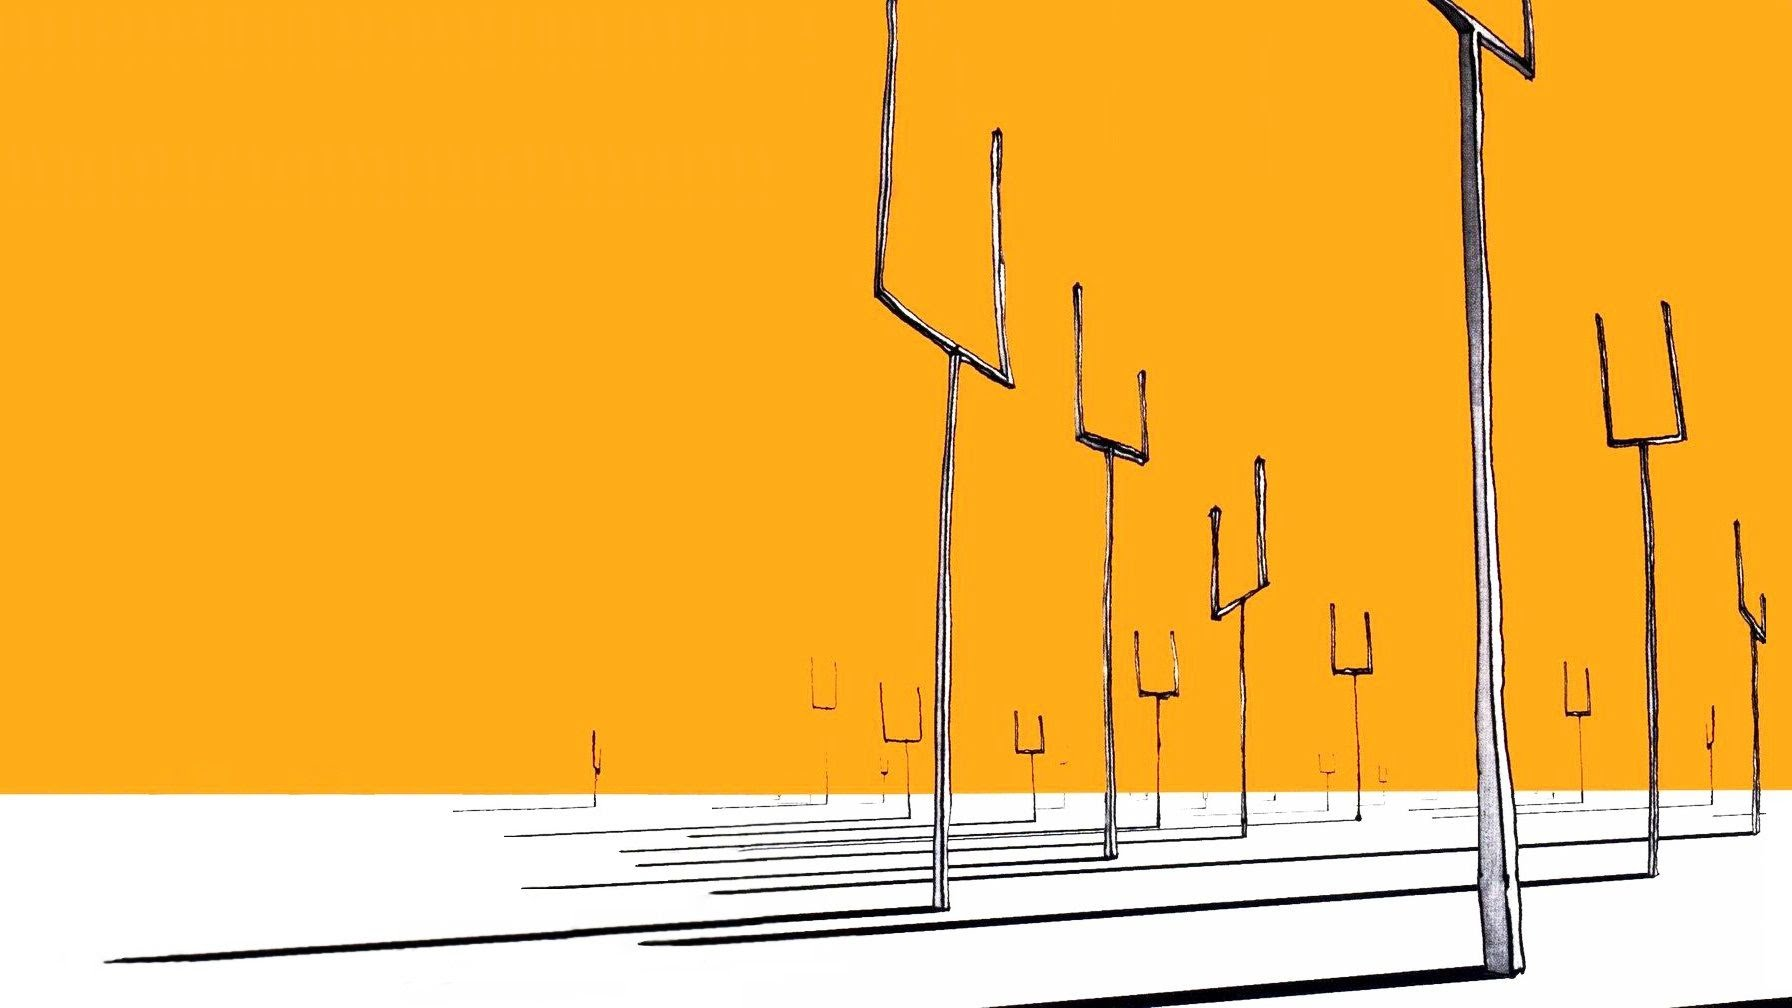
\includegraphics[width=10cm,height=6cm]{album_cover.jpg}
      \\\emph{Nota:} El autór de la portada es William Eagar.\label{fig:muse}
    \end{figure}
    A \begin{justifying}
      continuación se muestra el código del proyecto en su totalidad para posteriormente explicar las partes que lo conforman.\par
    \end{justifying}
    \vspace{\baselineskip}
    \begin{lstlisting}[language=JavaScript]
      // Elaborado con la biblioteca p5.js (Lenguaje capaz de ser ejecutado por navegadores web)
      // Declaracion de variables definidas(const)
      
      //PARAMETROS DE LORENZ
      const SIGMA = 10;
      const RHO = 28;
      const BETA = 8/3;
      
      //CONDICIONES INICIALES
      const X_0 = 0.11;
      const Y_0 = 1;
      const Z_0 = 1;
      
      //CAMBIO EN EL TIEMPO
      const DT = 1/60;
      const MAX_LEN = 60;
      
      // Variables globales
      let offset = 0;
      let p;
      let Lorenz;
      let prev;
      let next;
      let path = []; // Arreglo
      
      function setup() 
      {
        createCanvas(windowWidth, windowHeight, WEBGL); //lienzo
        colorMode(HSB, 100); // Cambia la forma en que p5.js interpreta los datos de color; Hub, Saturation and Brightness
        p = createVector(X_0, Y_0, Z_0);
      }
      
      function draw() 
      {
          //inicio del rgabador de gif
         // if(frameCount===1){ capturer.start(); }
      
        // Rotacion
        rotateY(frameCount * 0.005); //del eje Y
        rotateZ(frameCount * 0.005); //... Z
        scale(width/80); //permite modificar el tamanio de un elemento en el plano 
        background(15); // color de fondo
        strokeWeight(0.6); // Establece el ancho del trazo utilizado
        stroke(255); // Define el color trazado
        noFill(); // Sin relleno la figura formada
      
        Lorenz = createVector(
          SIGMA * (p.y - p.x),
          p.x * (RHO - p.z) - p.y,
          p.x * p.y - BETA * p.z 
        );
      
        Lorenz.mult(DT);
        p.add(Lorenz);
        path.push(p.copy());
      
        // Condicional para conocer si la longitud del path (ruta cookies) es mayor al valor de MAX_LEN ya definido
        if (path.length > MAX_LEN) 
        {
          path.splice(0, 1);
          ++offset;
        }
        
        prev = path[0];
      
        for (let i = 1; i < path.length; ++i)
        {
          //trazado y color de rectangulos
          fill(199+Math.random())
          rect(prev.x+noise(prev.x), prev.x+noise(prev.x),prev.y+noise(prev.y), prev.z*
          noise(prev.z));
          next = path[i];
          stroke(i + offset, 50, 50 - (path.length - i) * MAX_LEN); 
          prev = next;
        }
      }
      \end{lstlisting}
    \subsubsection*{Lineas 4-24: Variables Auxiliares}
    \addcontentsline{toc}{subsubsection}{Lineas 4-24: Variables Auxiliares}
    En \begin{justifying}
      estas lineas de código estamos definiendo los valores y variables auxiliares que se van a manejar a lo largo del programa.
      Aquellas que son declaradas como {\fontfamily{cmtt}\selectfont const} se van a mantener constantes a lo largo del programa,
      por ello los parámetros canónicos así como el valor de la diferencial ({\fontfamily{cmtt}\selectfont DT}) no se deben modificar.
      Aquellas que fueron declaradas con {\fontfamily{cmtt}\selectfont let} van a poder almacenar dinámicamente distintos datos alrededor
      de la ejecución de la animación.\par
    \end{justifying}
    \vspace{\baselineskip}
    \subsubsection*{Lineas 26-31: {\fontfamily{cmtt}\selectfont setup()}}
    \addcontentsline{toc}{subsubsection}{Lineas 26-31: {\fontfamily{cmtt}\selectfont setup()}}
    En esta parte, definimos el esquema de color que se va a utilizar a lo largo de la animación así como el procesamiento de imágen que se va a utilizar.
    Ambas nos permiten ilustrar y procesar la animación con distintos parámetros y equivalencias numéicas; HSB los procesa como grados de saturación mientras que
    WEB-GL es un protocolo de procesamiento de imágen tridimensional para los navegadores web. Aparte, se crea el vector que representará los valores iniciales
    de (\(x,y,z\)) del Atractor de Lorenz.\par
    \vspace{\baselineskip}
    \subsubsection*{Lineas 33-45: Rotación y Demás Detalles}
    \addcontentsline{toc}{subsubsection}{Lineas 33-45: Rotación y Demás Detalles}
    En \begin{justifying}
      estas sentencias estamos declarando la velocidad de rotación de los ejes \(y\) y \(z\) de la figura tridimensional a graficar; al reiniciar la animación,
    la figura base termina siendo la misma debido a que en conteo de los cuadros de la imágen siempre empieza en uno y aumenta acorde al FPS indicado (por defecto, 
    se renderiza a 60 FPS).\par
    \end{justifying}
    El \begin{justifying}
      resto de sentencias son otros aspectos de la configuración dinámica de la figura en cuestión:
    \begin{itemize}
      \item {\fontfamily{cmtt}\selectfont scale(width/80)}: encoje al objeto tridimensional acorde al valor del ancho de la ventana y lo escala por un factor de \({1\over80}\). Esto es para apreciar mejor a la obra.
      \item {\fontfamily{cmtt}\selectfont backround(15)}: fija el color del fondo a un tono grisaceo (acorde al sistema de color HSB).
      \item {\fontfamily{cmtt}\selectfont strokeweight(0.6)}: el grosor de las figuras auxiliares será \({6\over10}\) veces menos pronunciado (para los rectangulos).
      \item {\fontfamily{cmtt}\selectfont stroke(255)}: establece el color del trazo al 255 HSB.
      \item {\fontfamily{cmtt}\selectfont nofill()}: las figuras no tendrán color de relleno.
    \end{itemize}\par
    \end{justifying}
    Es \begin{justifying}
      de vital importancia que estas sentencias así como las restantes, se ejecutan en el método {\fontfamily{cmtt}\selectfont draw()} que ejecuta
    indefinidamente las sentencias dentro de este bloque, generando la animación esperada.\par
    \end{justifying}
    \vspace{\baselineskip}
    \subsubsection*{Lineas 47-55: Discretización de Lorenz}
    \addcontentsline{toc}{subsubsection}{Lineas 47-55: Discretización de Lorenz}
    Lo \begin{justifying}
      único que se está realizando es la conversión al Método de Euler en JavaScript del susodicho Atractor de Lorenz; la asignación de las ecuacioens con sus valores iniciales
    dados por el vector {\fontfamily{cmtt}\selectfont p} y subsecuentemente el almacenamiento de la ruta de memoria de dicha copia.\par
    \end{justifying}
    \vspace{\baselineskip}
    \subsubsection*{Lineas 58-64: Longitud de cookies}
    \addcontentsline{toc}{subsubsection}{Lineas 58-64: Longitud de cookies}
    La \begin{justifying}
      utilidad de éste fragmento de código es para generar otros valores que se puedan alimentar
      a la graficación de la animación deseada.\par
    \end{justifying}
    \vspace{\baselineskip}
    \subsubsection*{Lineas 66-75: Trazado de las Figuras Dentro de la Ruta del Atractor de Lorenz}
    \addcontentsline{toc}{subsubsection}{Lineas 66--75: Trazado de las Figuras Dentro de la Ruta de Lorenz}
    Este \begin{justifying}
      es el fragmento más importante del código, debido a que se generan los rectangulos, sus medidas y sus colores,
    así como el grosór del contorno de dichos rectangulos acorde a los valores (en el momento del cálculo) del Atractor
    de Lorenz en ese instante de tiempo.\par
    \end{justifying}
    El \begin{justifying}
      ciclo iterativo es para utilizar el valor del índice como otro parámetro para laconstrucción de los rectangulos; dentro de éste
      declaramos el relleno de la figura, y llamamos a la función {\fontfamily{cmtt}\selectfont rect()} que construye los rectangulos con cuatro parámetros
      , los primeros dos corresponden a la ubicación de su esquina superior derecha respecto al plano \(xy\) y los últimos dos corresponden a lo alto y ancho.
      En ámbas se utiliza la función {\fontfamily{cmtt}\selectfont noise()} que genera un valor aleatorio menos ``brusco'' que la función {\fontfamily{cmtt}\selectfont random()}, 
      permitiendo variaciones más naturales y estéticas de tamaño (Figura ~\ref{fig:ruido}).\par%citar la imagen de abajo
    \end{justifying}
    \begin{figure}[H]
      \centering
      \caption{Ruido Perlin en contraste con Random}
      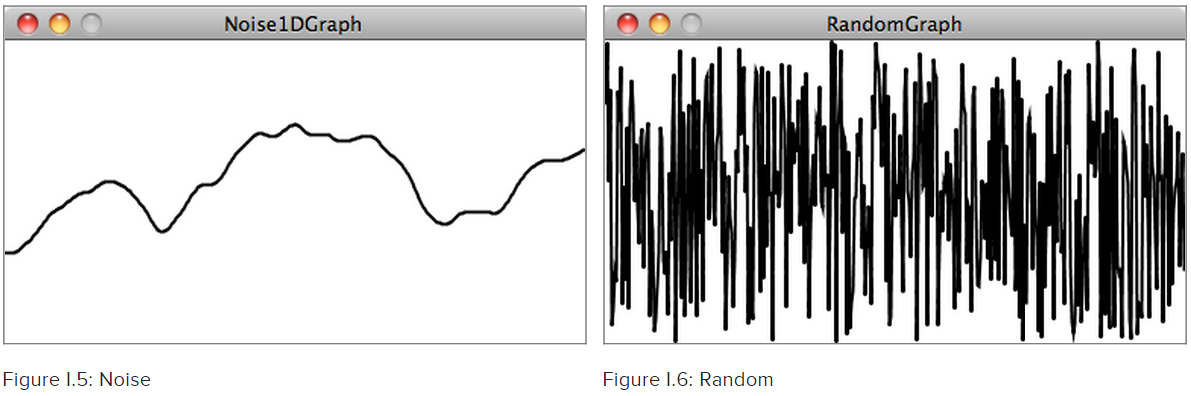
\includegraphics[width=10cm,height=6cm]{perlin_vs_random.png}
      \\\emph{Nota:} Los valores de Random denotan cambios bruscos. Tomado de StackOverFlow.\label{fig:ruido}
    \end{figure}
    Finalmente, \begin{justifying}
      el resto de las sentencias actualiza los valores de las variables y permite el color del trazo con variaciones leves que combinan con la paleta de colores
    de la obra final, que se muestra en la Figura ~\ref{fig:proyecto}.\par %citar la imagen de abajo
    \end{justifying}
    \begin{figure}[H]
      \centering
      \caption{Instante de la animación del proyecto}
      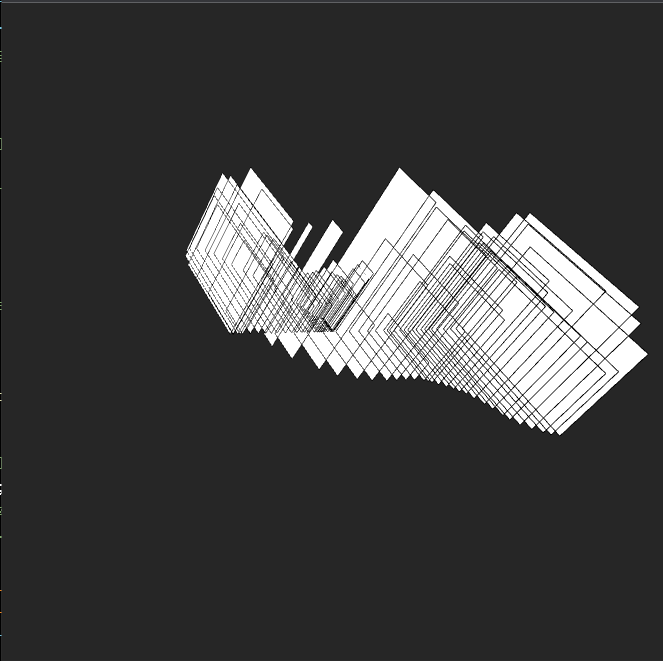
\includegraphics[width=10cm,height=8cm]{prueba.png}
      \\\emph{Nota:} Autoría Propia.\label{fig:proyecto}
    \end{figure}
    \vspace{\baselineskip}
    \section*{Conclusiones Preliminares}
    \addcontentsline{toc}{section}{Conclusiones Preliminares}
    El \begin{justifying}
      haber iniciado con la cuestión de poder aplicar un sistema caótico como el Atractor de Lorenz a las artes visuales, nos permitió
    explorar las distintas tangentes expuestas a lo largo del documento y poder probar el lado artístico de estas herramientas. La 
    parte programática con ayuda de Processing fue bastante simple ya que la sintáxis era similar a lo que ya habiamos manejado a lo largo de la carrera,
    aunque hemos de admitír que el resultado final fue concebido por una constante prueba muy pragmática que nos permitió observar resultados muy
    distintos a lo que se presenta como el ``resultado final'' del proyecto, por lo que aún hay muchas vertientes que se pueden explorar dentro del 
    código fuente, que permite sentar un precedente para seguir experimientando con la graficación y tener un acercamiento más visceral ante el proceso
    de creación artística que nos dió una perspectiva sobre la predominancia de la habilidad creatíva de los artístas visuales en contraste de las herramientas
    con las cuales crean árte.\par
    \end{justifying}
    \vspace{\baselineskip}
    
    \newpage   
    % Referencias
    \renewcommand\refname{\textbf{Referencias}}
    \bibliographystyle{ieeetr}
    \bibliography{referencias}
\end{document}